\chapter[Studies]{Study of the existing}
 \par This part will be splitted in 2 because the subjects are totally differents. I am going to talk first about the helmet, that required a bit less than 1 month of test and studies. I will explain the procedures in the next chapter. 
	
	\section{Helmet study}	
	\subsection{Helmet itself}
	\par I began my study by acquiring some knowledges about the helmet itself. It has been release in the end of 2013, build for harsh condition, its price makes it unaccessible for the public. The army and building companies saw a good opportunity in this technologie to ease the work by bringing communication into the field.
	\par The helmet is equiped with a batterie, Wi-Fi and blutooth connections, a camera and it can be wear under the work helmet. Everything is voice commanded and very responsive thanks to Motorola's work. Windows CE 6.0 is used on the last release of the helmet image. It is good for the next section to understand that the booting system and the update system of windows CE are related. That means that you can change the file system for an update but it is windows itself that validate and copy the files on the intern memory from the SD card.
	\subsection{Embedded systems}
	\par I learned a lot about embbeded system, mainly on the boards and all the peripherics. In our case, the components inside the helmet are not known and not published on the Internet. Pierluigi contacted the company that brought us the helmet but they couldn't tell us which board was used in the helmet. I guessed which TI technology it was because the datasheet reference a TI OMAP 3 microprocessor. 
	\par That is mainly why I put my effort on the "ISEE – IGEP COM MODULE" built in with a TI OMAP 3 processor. It was at the state of the art when the helmet released and the smallest board with this processor. It corresponds well with the size of the hardware slot. In any case, if the linux kernel is compatible with the processor a cross compiled file system should boot and at least it should show an image on the screen.
	
	\subsection{Cross-compilation}
	\subsubsection{Description}
	\par The cross-compilation is compilation\footnote{Process that generate binary file for a specific achitecture.} for a different achitecture than the architecture that makes the computations. In the figure~\ref{cross} you can see that the source code can be compiled for different architectures. The aim here was to compile a Linux kernel compatible with TI OMAP 3 processors from an Intel x86 machine.
	\begin{figure}[h]
		\begin{center}
			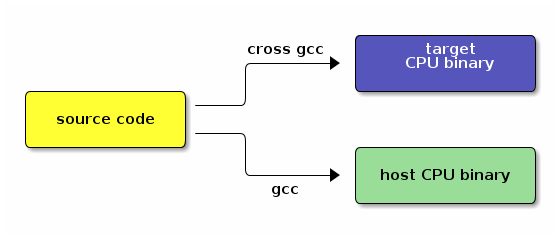
\includegraphics[scale=0.5]{images_not_compressed/cross-compile.png}
			\label{cross}
			\caption{Cross compilation and compilation difference}
		\end{center}
	\end{figure}


\subsubsection{Toolchain}
	
	\par A toolchain is a set of distinct software development tools that are linked (or chained) together by specific stages such as GCC, binutils and glibc (a portion of the GNU Toolchain)\cite{Toolchain}.
	\par A toolchain requires binutils such as assembler and linker, that produces the binaries. Also compilers for deferent languages like C, C++, Java etc, that transforms any language into another. A C library to gain access to kernel calls and a debugger that can be used or not during the compilation. We can see well on the diagram \ref{compchain} (from avrfreaks.net's forum)  where each composant is located :
	\begin{figure}[ht]
		\begin{center}
			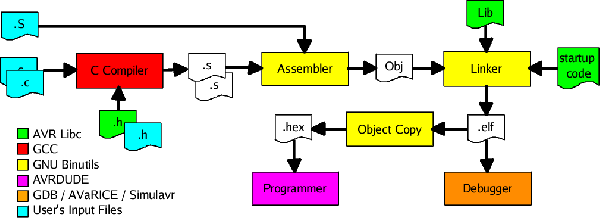
\includegraphics[scale=0.5]{images_not_compressed/compchain.png}
			\label{compchain}
			\caption{Cross compilation and compilation difference}
		\end{center}
	\end{figure}
	
	
	\subsubsection{Process}
	\par The cross tool chain is capable of compile a Linux kernel for a lot of achitectures. Of course it requires a long time to compile the toolchain and then cross compile the kernel to get the binaries but it is cost effective. The time necessere to compile the toolchain and the kernel on the TI OMAP 3 would be longer.

		
	\section{Pattern recognition study}
	\subsection{OpenCV}
	
		\begin{wrapfigure}[4]{l}{2cm}
	\vspace{-7mm}
	
\includegraphics[width=2cm]{images_not_compressed/opencv_logo.png}
	\end{wrapfigure}
	\par OpenCV is an image analysis and synthesis library that brings all the necessary for video and photo analysis. Introduced in 2000, it is now used a lot in the fields that require image analysis.
 It is built around a modular system that allows users to install the library depending on their needs.
 Except the non free module, the library is licensed BSD which means that we can reuse and modify all the components freely.
 In this document I will talk more about precise modules of OpenCV as a base and features2d modules.
	
	\subsection{Existing code}
	
	\par To get some examples of code and see how it works I simply looked at the OpenCV tutorials that are available on the internet. For example check~\hyperlink{opencv}{it in the annexe section}. It brings a simple way to extract a pattern and make the homography to draw the corners with lign OpenCV function.
	
	\subsubsection{Key points}
	\par SIFT points are points of interest in the image. They give the position of an area where all the pixels have approximately the same properties. Using the Laplacian of Gaussian of the image, maxima and minima which corresponding to these areas can be extracted.
	\par The biggest advantage of these areas is the invariance in transformation like rotation, scaling and translation. Pattern detection algorithm based on this points are insensitive in term of scale and rotation. That is mainly why it has been chosen for this application. By the time that the resolution of the pattern must be over an acceptable threshold. We can move and rotate the object without altering the detection.
	
	\subsubsection[Descriptor]{SIFT Descriptor}
	\par The descriptors are computed from the key points. The descriptors associated with the SIFT key points are locally oriented histograms around a SIFT key point \cite{AM}:
	
	\begin{itemize}
			\item We divide space around each key point (x, y) in N\ts{2} squares of 4 by 4 \item We compute the gradient \begin{math}G_{x}(a,b,\sigma)\end{math}, \begin{math}G_{y}(a,b,\sigma)\end{math} for the 4 by 4 by N\ts{2} points (a, b)

		\item For each 4 by 4 square, we compute a histogram of the orientations in 8 directions, multiplying by: (1) the module of the gradient (2) the inverse of the distance to the key point (x, y).
 \item To be invariant in rotation: the local orientation of the key point \begin{math} \theta(x,y) \end{math} is used as the origin (null orientation) of the histograms.		
	\end{itemize}
	
	
	\subsubsection{Homography}
	\par  Just to give a simplified idea, the familiar Cartesian plane is composed by a set of points which have a one-to-one correlation to pairs of real numbers, i.e. X-Y on the two axis\cite{Homography}.
	\par In our case, the points are the key points extracted. By generating the homography matrix, we can transform the corners of our image to 4 other points representing the position of the object on the scene\cite{TutoHomography}.
	
	\begin{wrapfigure}[12]{r}{10cm}
			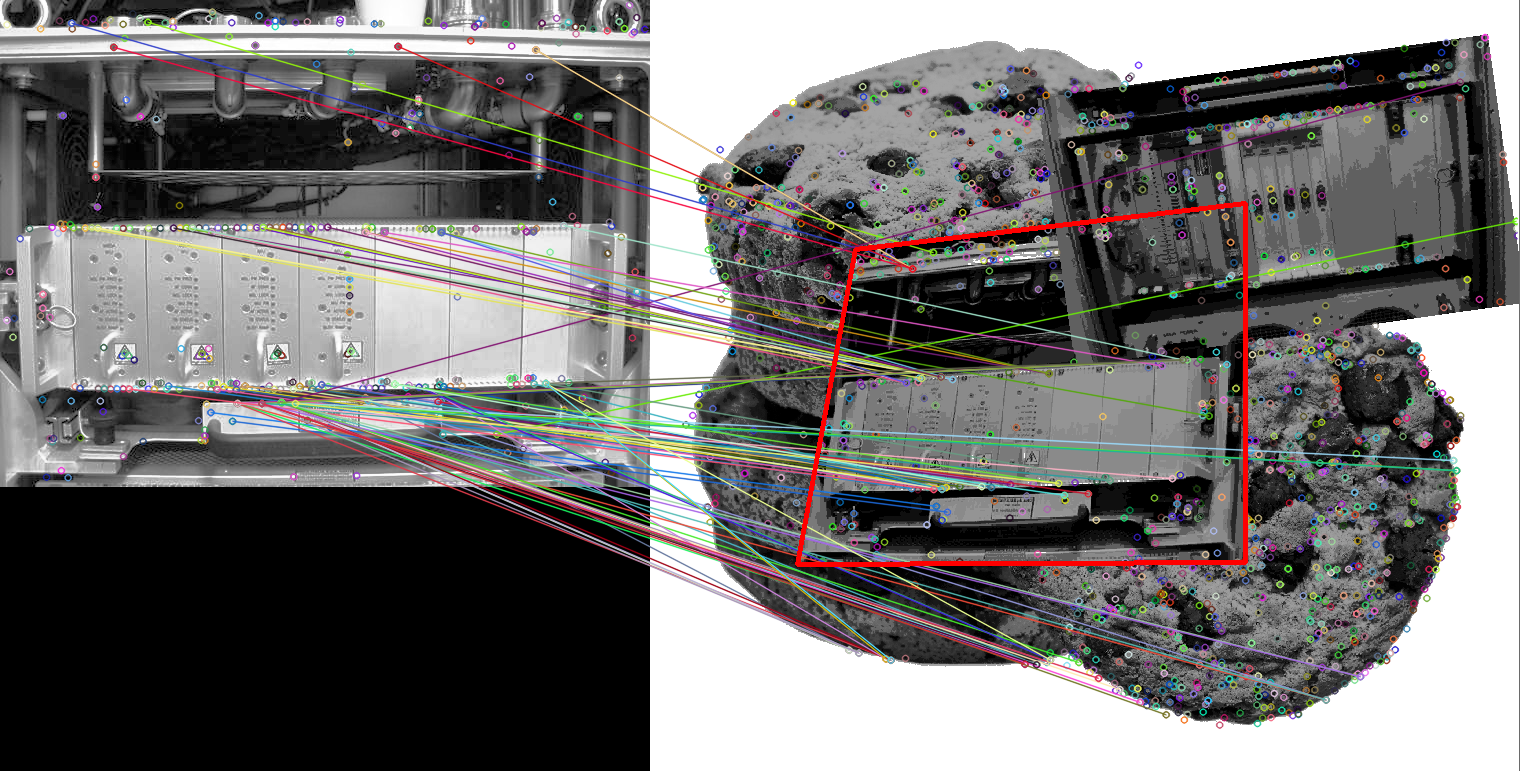
\includegraphics[width=10cm]{images_not_compressed/showHomography.png}
			\caption{Homography with a corner hidden with openCV}
	\end{wrapfigure}
	\par On the image behind we can see that the homography doesn't depend on the corners. All the key points can be a base for analize. And using the perspective transform of OpenCV that multiplies the corners by the homography matrix. We obtain the position of the corners on the captured image.
